\chapter{RTL-to-GDSII Design Flow Using OpenLane2}
\label{chap:rtl_to_gdsii}

This chapter describes the complete ASIC implementation flow used to transform the verified RTL design into a manufacturable GDSII layout. The implementation was performed using the open-source OpenLane2 flow, which integrates industry-standard tools for synthesis, physical design, routing, timing optimization, and physical verification.

The UART IP core was implemented using the SkyWater SKY130 open-source Process Design Kit (PDK). The design flow begins with synthesizable Verilog RTL and automatically progresses through logic synthesis, floorplanning, placement, clock tree synthesis, routing, and physical verification before generating the final GDSII layout.

%%%%%%%%%%%%%%%%%%%%%%%%%%%%%%%%%%%%%%%%%%%%%%%%%%%%%%%%%%%%%%%%%%%%%%%

\section{OpenLane2 Design Flow}

OpenLane2 provides an automated RTL-to-GDSII implementation flow by integrating multiple open-source EDA tools into a unified framework. The complete design flow used in this project is illustrated in Figure~\ref{fig:openlane_flow}.

\begin{figure}[!htbp]
\centering
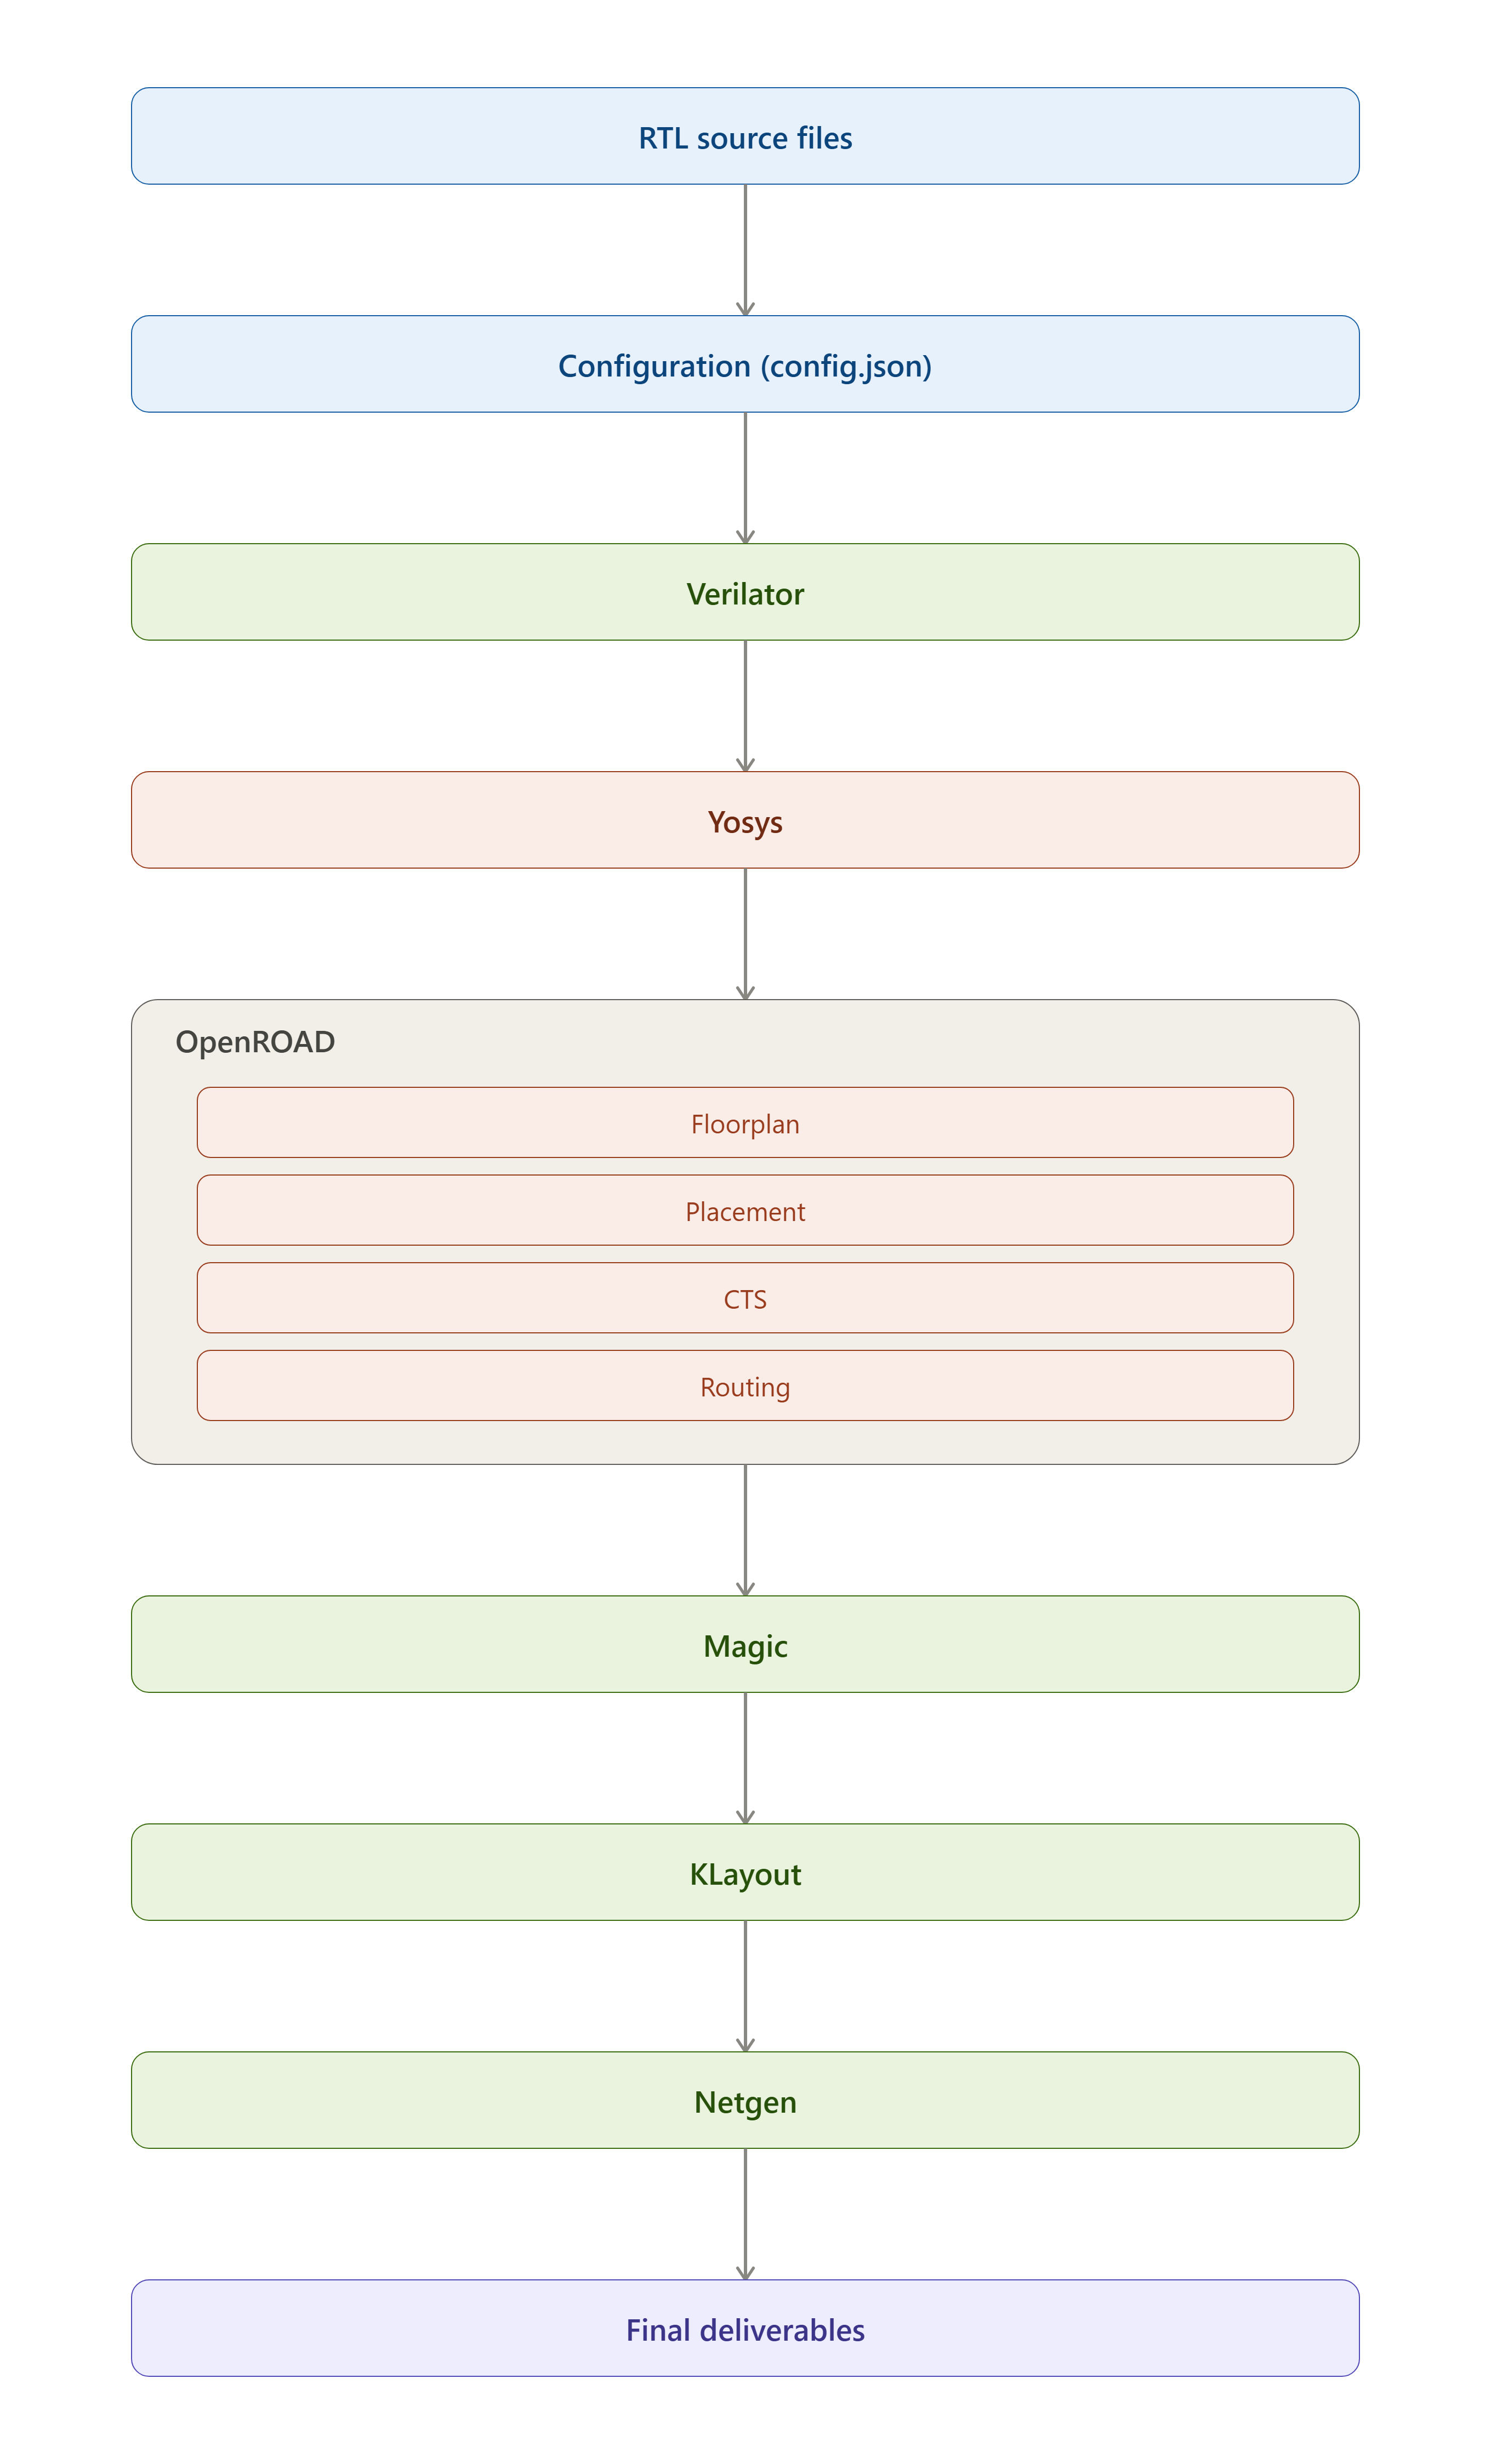
\includegraphics[width=0.85\textwidth]{images/openlane2_internal_workflow.png}
\caption{Complete RTL-to-GDSII implementation flow using OpenLane2.}
\label{fig:openlane_flow}
\end{figure}

The major stages of the implementation flow are summarized below.

\begin{table}[!htbp]
\centering
\caption{Major stages of the OpenLane2 ASIC design flow}
\label{tab:openlane_stages}
\begin{tabular}{ll}
\toprule
Stage & Description\\
\midrule
RTL Design & Verilog HDL implementation\\
RTL Linting & Design rule and syntax checking\\
Logic Synthesis & RTL converted into gate-level netlist\\
Floorplanning & Core and I/O planning\\
Placement & Standard cell placement\\
Clock Tree Synthesis & Clock distribution network generation\\
Routing & Signal interconnection\\
Physical Verification & DRC and LVS verification\\
GDSII Generation & Final layout generation\\
\bottomrule
\end{tabular}
\end{table}

%%%%%%%%%%%%%%%%%%%%%%%%%%%%%%%%%%%%%%%%%%%%%%%%%%%%%%%%%%%%%%%%%%%%%%%

\section{Project Directory Structure}

The UART project was organized into separate directories for RTL source files, testbenches, configuration files, simulation outputs, reports, and implementation results.
\begin{verbatim}
uart_asic_ip/
|
|-- rtl/
|   |-- uart_top.v
|   |-- uart_tx.v
|   |-- uart_rx.v
|   `-- baud_generator.v
|
|-- tb/
|
|-- waveforms/
|
|-- sim/
|
|-- config.json
|
|-- runs/
|
|-- reports/
|
|-- logs/
|
`-- results/
\end{verbatim}

This directory organization simplifies project management and separates design sources from generated implementation files.

%%%%%%%%%%%%%%%%%%%%%%%%%%%%%%%%%%%%%%%%%%%%%%%%%%%%%%%%%%%%%%%%%%%%%%%

\section{Design Configuration}

OpenLane2 uses a \texttt{config.json} file to define the design-specific implementation parameters. This configuration specifies the top module, RTL source files, target PDK, clock information, and implementation constraints.

The primary configuration parameters used in this project are summarized in Table~\ref{tab:config}.

\begin{table}[!htbp]
\centering
\caption{Important OpenLane2 configuration parameters}
\label{tab:config}
\begin{tabular}{ll}
\toprule
Parameter & Purpose\\
\midrule
DESIGN\_NAME & Top module name\\
VERILOG\_FILES & RTL source files\\
CLOCK\_PORT & Primary clock input\\
CLOCK\_PERIOD & Target clock period\\
PDK & SkyWater SKY130 PDK\\
STD\_CELL\_LIBRARY & SKY130 standard cells\\
\bottomrule
\end{tabular}
\end{table}

%%%%%%%%%%%%%%%%%%%%%%%%%%%%%%%%%%%%%%%%%%%%%%%%%%%%%%%%%%%%%%%%%%%%%%%

\section{RTL Linting Using Verilator}

Before synthesis, the RTL design was analyzed using Verilator to detect syntax errors, unsupported constructs, signal mismatches, and coding issues.

RTL linting improves design quality by identifying potential implementation problems before the synthesis stage. Successful completion of RTL linting ensures that the Verilog source files are suitable for logic synthesis.

%%%%%%%%%%%%%%%%%%%%%%%%%%%%%%%%%%%%%%%%%%%%%%%%%%%%%%%%%%%%%%%%%%%%%%%

\section{Logic Synthesis Using Yosys}

Logic synthesis converts the behavioral Verilog description into a technology-mapped gate-level netlist using the SkyWater SKY130 standard cell library.

The synthesis process includes RTL parsing, hierarchy checking, logic optimization, technology mapping, and netlist generation.

Figure~\ref{fig:yosys_flow} illustrates the major synthesis stages.

\begin{figure}[!htbp]
\centering
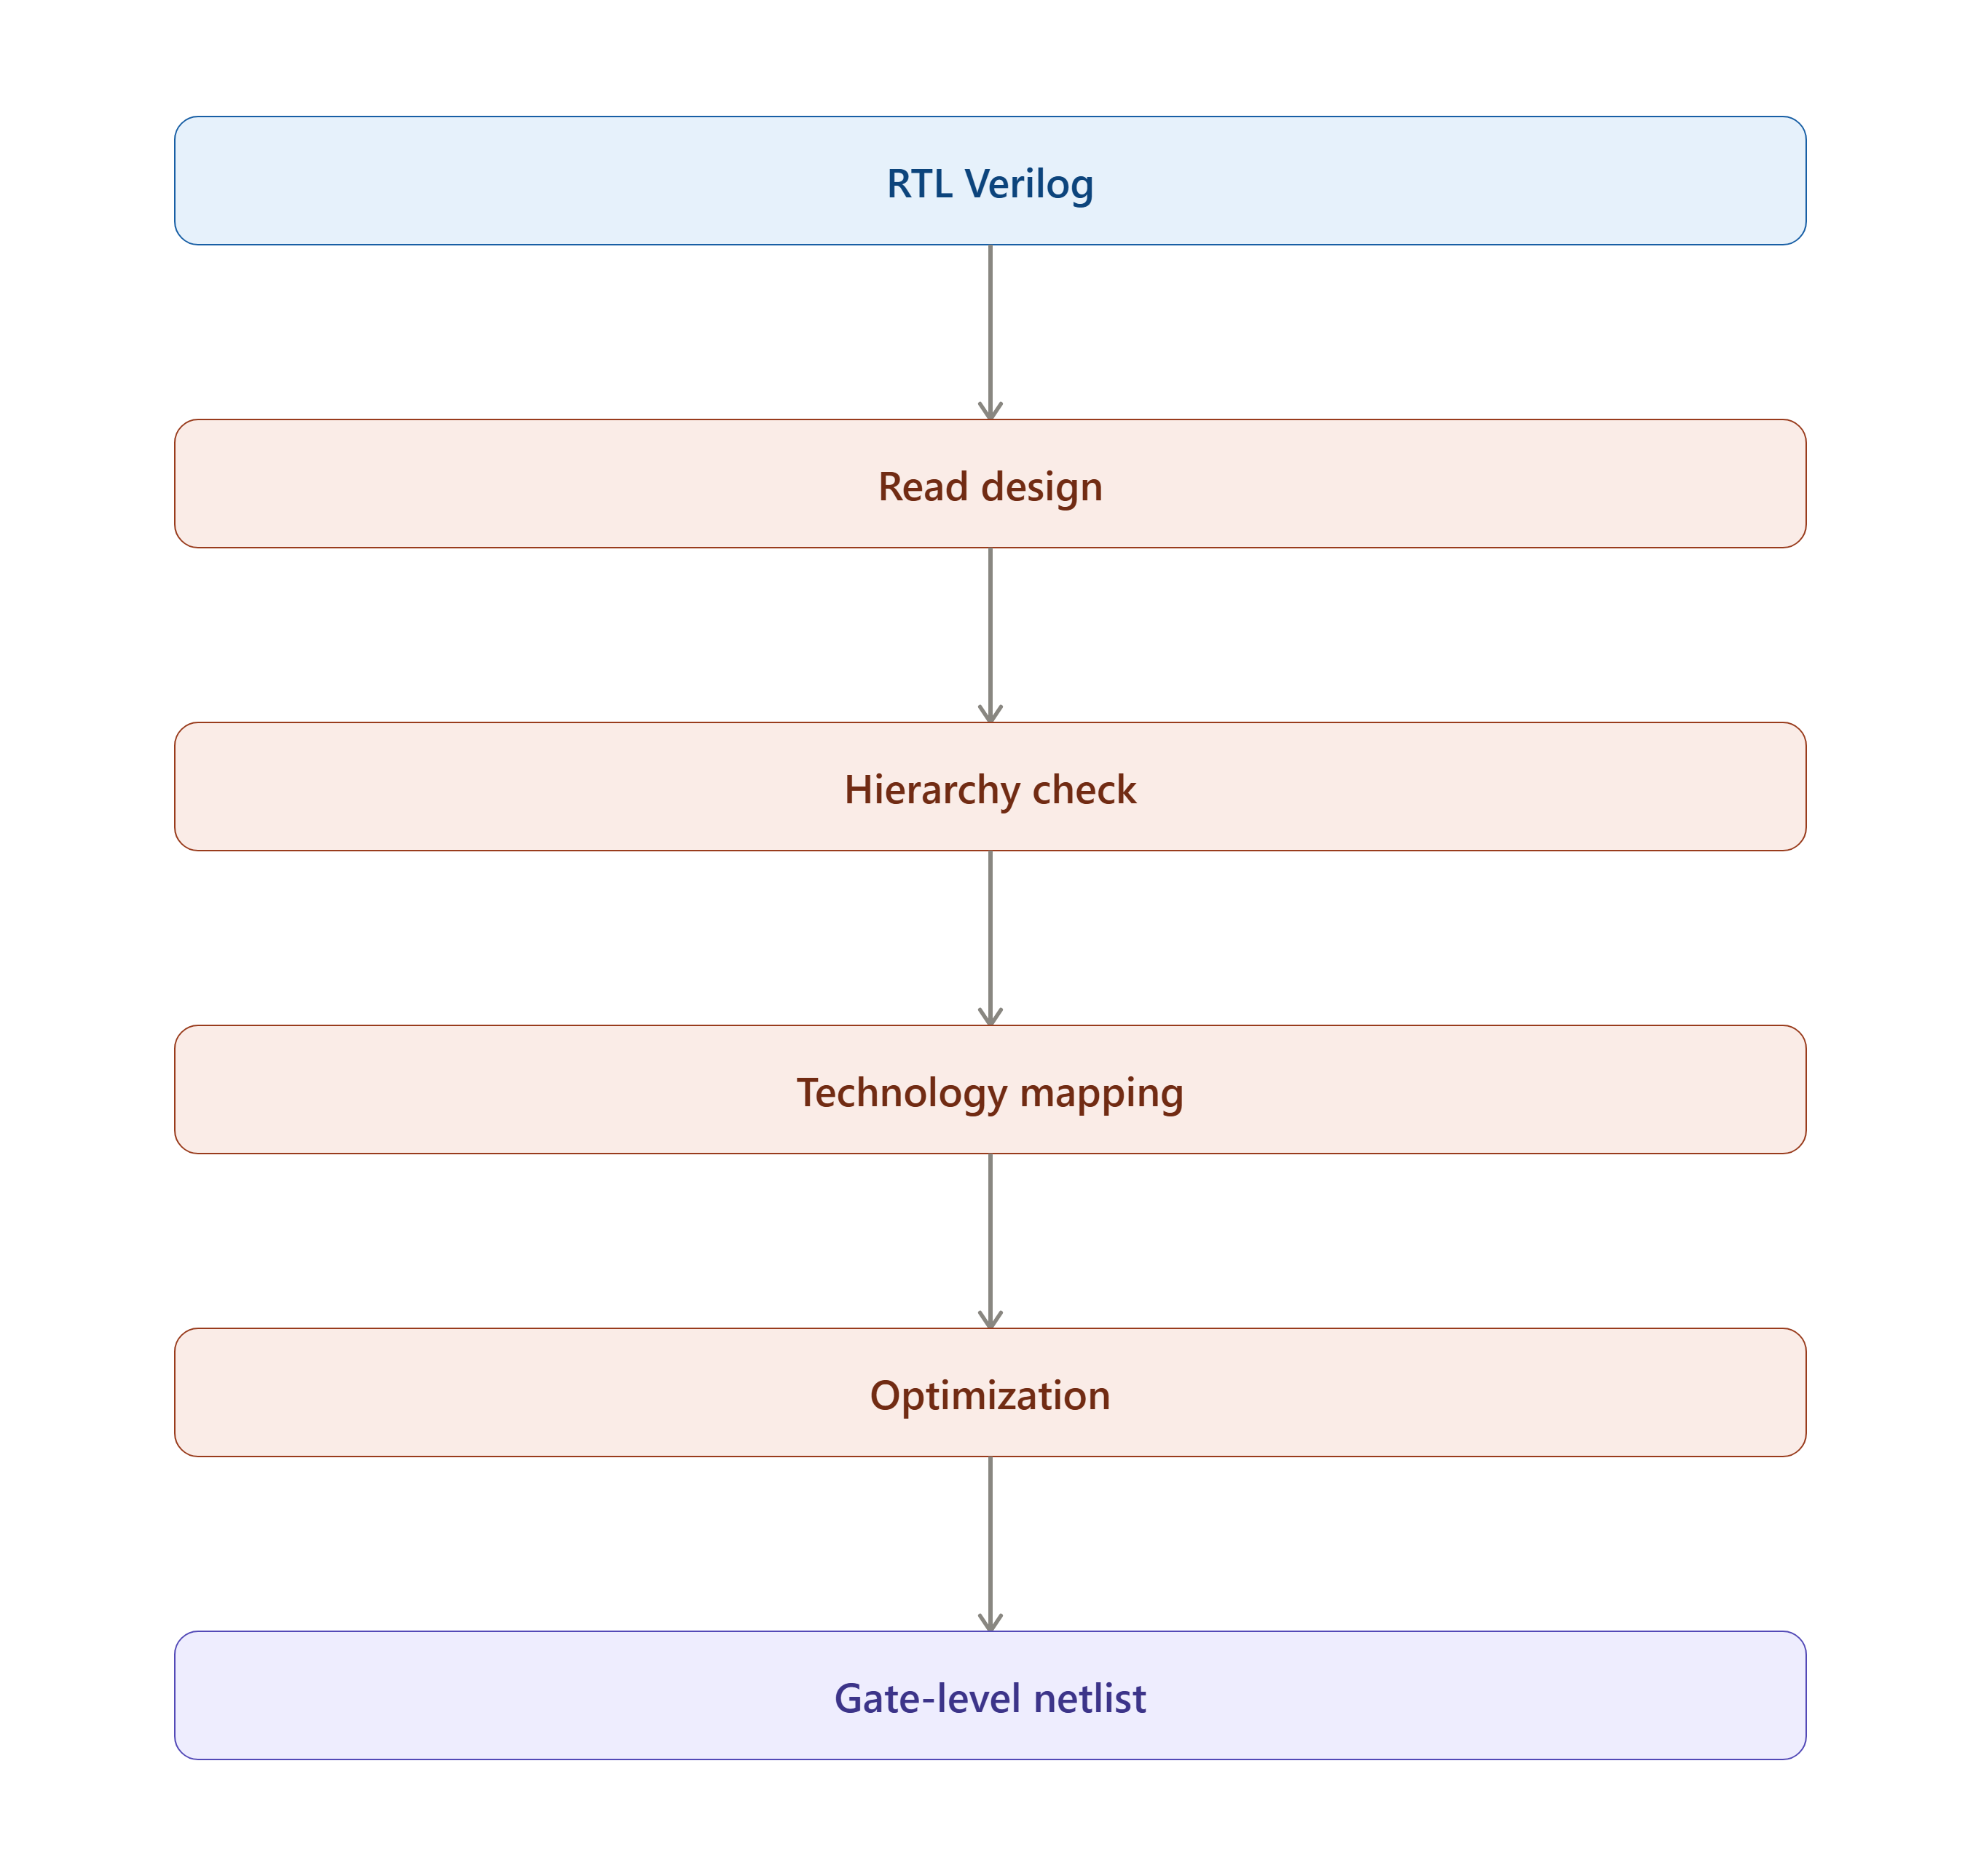
\includegraphics[width=0.78\textwidth]{images/synthesis_flow.png}
\caption{Logic synthesis flow performed using Yosys.}
\label{fig:yosys_flow}
\end{figure}

The synthesized gate-level netlist generated during this stage serves as the input for the subsequent physical design stages.

%%%%%%%%%%%%%%%%%%%%%%%%%%%%%%%%%%%%%%%%%%%%%%%%%%%%%%%%%%%%%%%%%%%%%%%

\section{Complete OpenLane2 Implementation Pipeline}

The overall implementation pipeline combines all open-source tools into a single automated ASIC design flow. Each tool performs a dedicated task and passes its output to the next stage until the final GDSII layout is produced.


Table~\ref{tab:eda_tools} summarizes the primary EDA tools used throughout the implementation flow.

\begin{table}[!htbp]
\centering
\caption{Open-source EDA tools used in this project}
\label{tab:eda_tools}
\begin{tabular}{ll}
\toprule
Tool & Function\\
\midrule
Verilator & RTL linting and design checking\\
Yosys & Logic synthesis\\
OpenROAD & Physical implementation\\
Magic & Layout generation and DRC\\
KLayout & Layout visualization and DRC\\
Netgen & Layout versus schematic (LVS) verification\\
\bottomrule
\end{tabular}
\end{table}

The outputs generated during each stage of the implementation flow are summarized in Table~\ref{tab:outputs}.

\begin{table}[!htbp]
\centering
\caption{Generated outputs during RTL-to-GDSII implementation}
\label{tab:outputs}
\begin{tabular}{ll}
\toprule
Stage & Output\\
\midrule
RTL Design & Verilog source files\\
Logic Synthesis & Gate-level netlist\\
Floorplanning & Floorplan DEF\\
Placement & Placed DEF\\
CTS & Clock tree\\
Routing & Routed DEF\\
Physical Verification & DRC and LVS reports\\
Final Output & GDSII layout\\
\bottomrule
\end{tabular}
\end{table}

The detailed implementation of floorplanning, placement, clock tree synthesis, routing, and physical verification is presented in the following chapters.